
\section{Results}
\label{sec:results}

To demonstrate the effectiveness of the nested iterative algorithm, we utilize both analytical closed form functionals and real world data in both 1-D and 2-D. A list of the problems tested is given below.

% Explain about the common problem datasets that we are going to be using and why they have been chosen.

\begin{enumerate}
	\item Synthetic data: sinc($x$)=$\frac{sin(x)}{x}$ functional on $\Omega \in [-4, 4]$
	\begin{itemize}
		\item 1-D: Q = (sinc($x$) + sinc(2*$x$-1) + sinc(3*$x$+1.5)), 
		\item 2-D: Q = (sinc($\sqrt{x^2+y^2}$))
	\end{itemize}
	\item S3D: This is a 3-D turbulent combustion dataset generated by an S3D simulation \cite{chen-s3d-2009} of fuel jet combustion in the presence of an external cross-flow. 
	% \item Nek5000: A 3-D dataset from CFD simulation with velocity magnitude as the solution profile
	\item CESM: A 2-D Community Atmosphere Model climate model dataset on a sphere with 3600x1800 resolution
\end{enumerate}


\subsection{1-d Results}\label{AA}

%Problem setups
%\begin{itemize}
%  \item Sine
%  \item Sinc
%  \item S3D
%%  \item Dow-Jones historical daily data
%\end{itemize}

\begin{itemize}
	\item Use the first two problems to measure convergence in parallel as number of domains increase
	\item Talk about adaptivity and resolution of data even for highly varying problem data.
\end{itemize}

\subsubsection{Adaptive Error Convergence and Verification}

The 1-d implementation of the ASM iterative solver was applied to the sinc problem. An initial input problem size of 500 points were evaluated and MFA representation for the resulting profile was computed on 4 subdomains. The solution profile, along with the control point locations from the adaptive computation are shown in \fig{fig:since-adaptive-1d}. We utilized the residual definition shown in \eqt{eq:nonlinear-residuals} with a $G_1$ constraint to be satisfied along all subdomain interfaces. The \fig{fig:since-adaptive-1d-b} and \fig{fig:since-adaptive-1d-c} present the zoomed in reconstruction of the approximation near the interface between $\Omega_2$ and $\Omega_3$ before and after the ASM iterations are converged. The discontinuous representation of data when performing independent, unconstrained subdomain solves are converged to satisfy the constraints after only 3 iterations, with nearest neighbor exchange of control point data at the interfaces.

\begin{figure}
	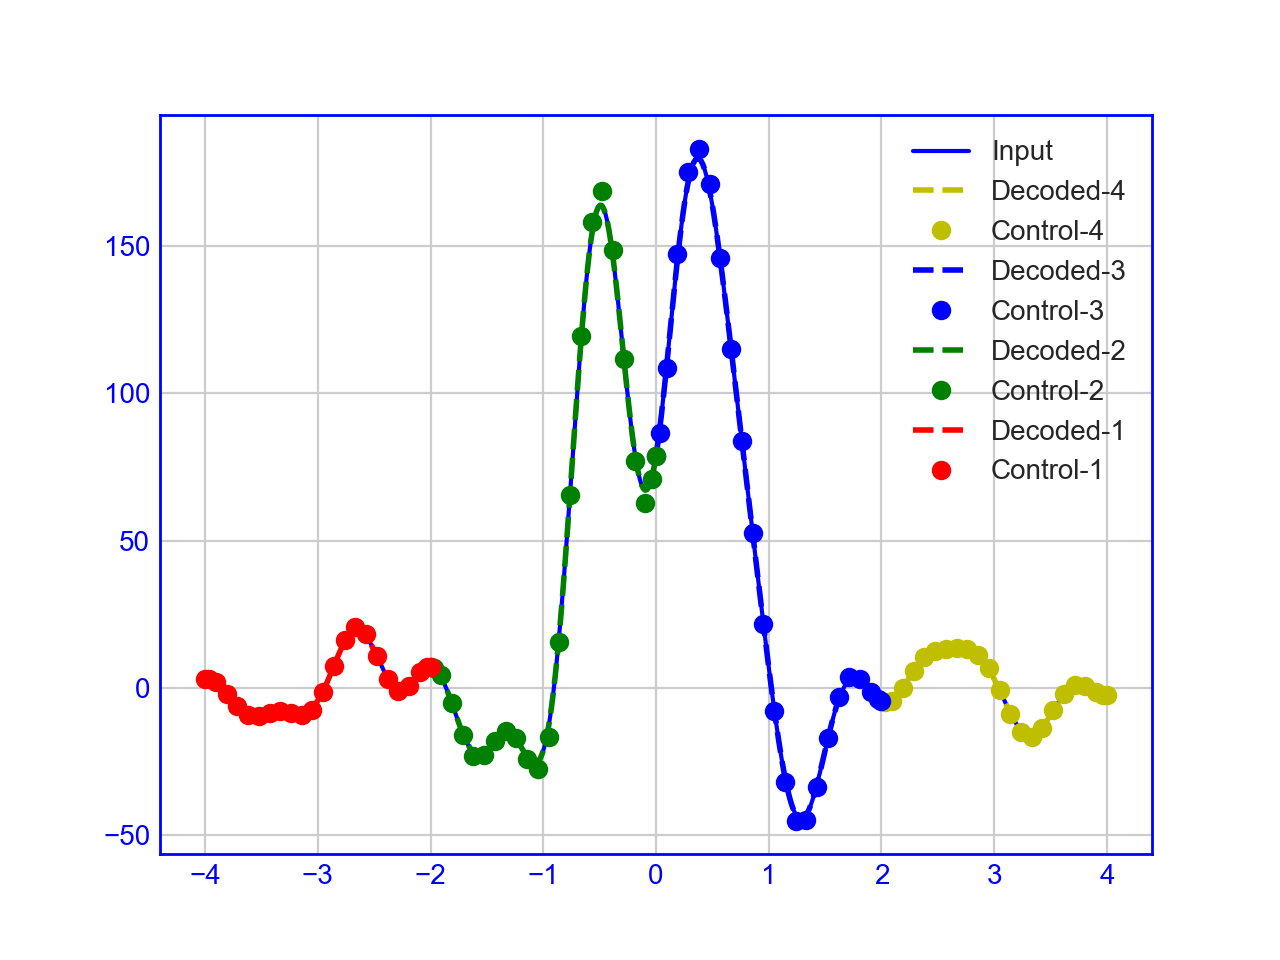
\includegraphics[width=0.48\textwidth]{figures/sinc-1d-profile}
	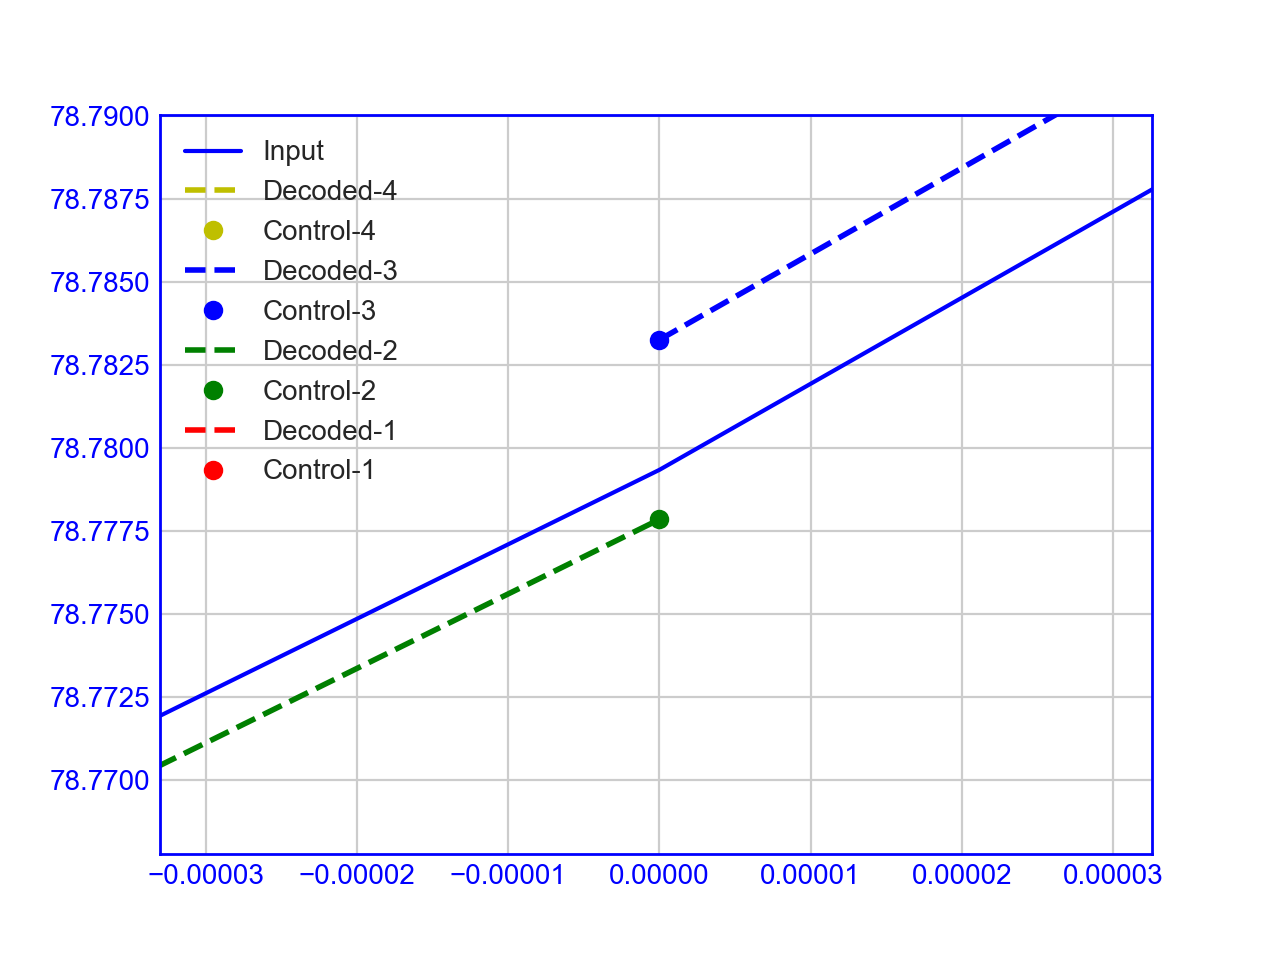
\includegraphics[width=0.24\textwidth]{figures/sinc-1d-discontinuous}
	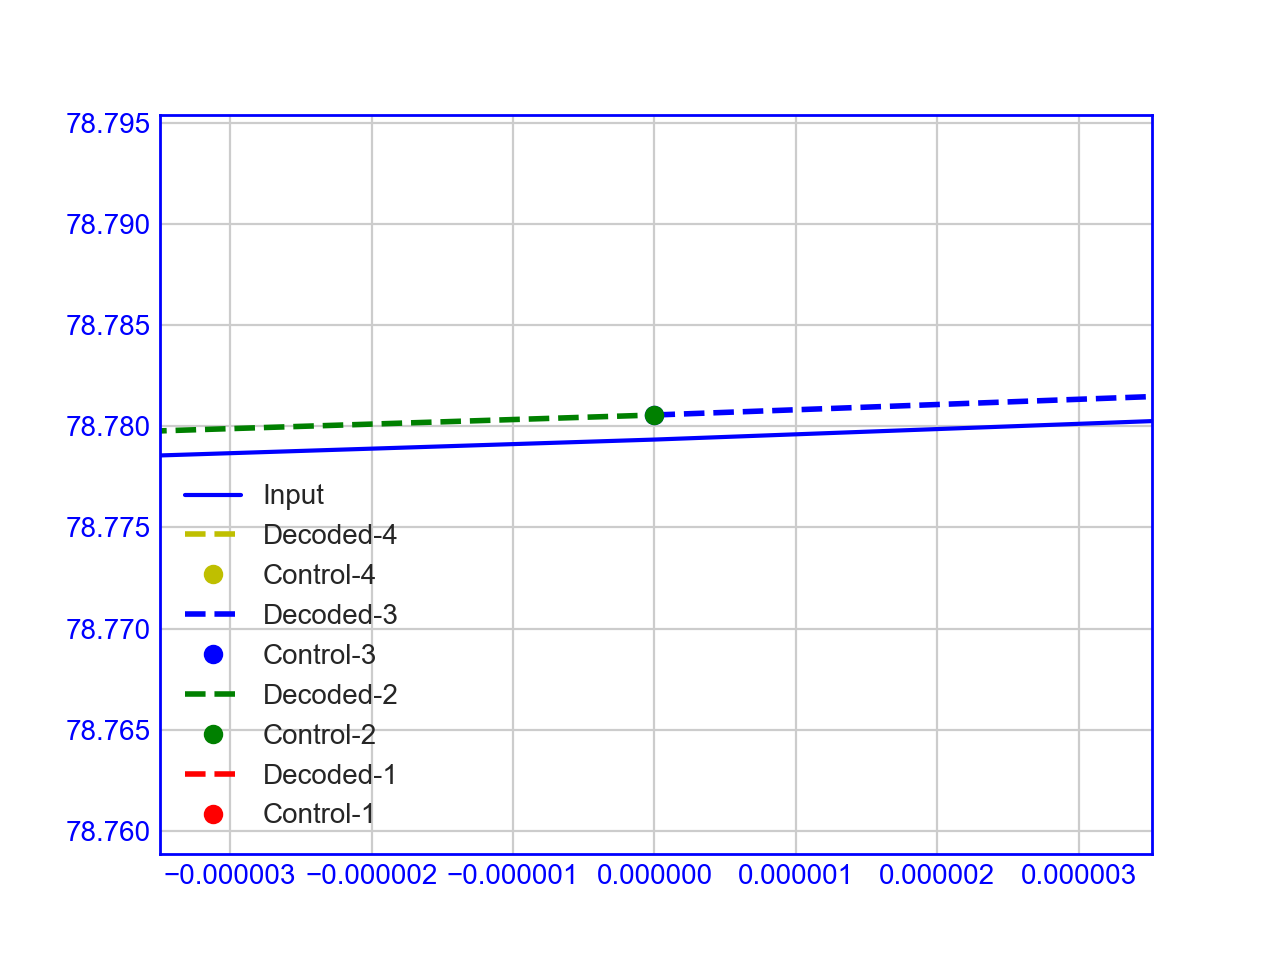
\includegraphics[width=0.24\textwidth]{figures/sinc-1d-continuous}
	\caption{1-D analytical sinc dataset with 501 input points: adaptive MFA on 4 subdomains with $10^{-4}$ tolerance}
	\label{fig:since-adaptive-1d}
\end{figure}


\subsubsection{Overlap Experiments in 1-D}

In this 1-D experiment on the closed form sinc function shown in \sect{sec:results}, we utilize the decoded residual minimization with the ASM-Krylov solver combination, and increase the amount of overlap in the input points to look at convergence speed. We measured the global $L_2$ error convergence along with the total cost in terms of outer iteration to compute the constrained control point locations. In this analysis, adaptivity in the individual subdomains was explicitly turned off so as to maintain a constant ratio of input points to control points per subdomain, as overlap region is extended in the subdomains on both the left and right sides.

\fig{fig:decoded-overlap-data-performance} shows the global $L_2$ norm of the net error in the decoded residual, as the number of subdomains are increased. With no overlap regions, where only the interface data is shared, the total ASM iterations needed to satisfy convergence, and the net error increase monotonically with $n_s$. As the overlap size becomes larger, for $\Delta=32$ and $\Delta=64$, the error growth and the iterations required remain much more bounded. This result closely matches the DD ASM preconditioning theory often applied in PDE solvers \cite{smith-ddm, lions-asm, gander-rasm}. It also shows that the ASM iterative scheme can be accelerated more efficiently, and scalably used as a solver without linear complexity on O($n_s$).

\begin{figure}
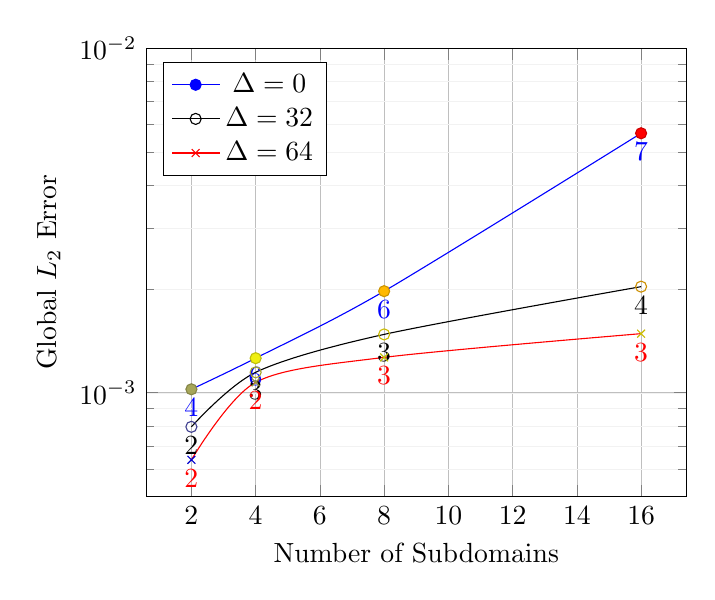
\begin{tikzpicture}

\begin{semilogyaxis}[
legend pos= north west,
ymin = 0.0005, ymax = 0.01,
xlabel=Number of Subdomains,
ylabel=Global $L_2$ Error,
nodes near coords*={\Label},
visualization depends on={value \thisrow{label} \as \Label},
grid=both,
grid style={line width=.1pt, draw=gray!10},
major grid style={line width=.2pt,draw=gray!50},
axis line style={latex-latex},
%axis lines=middle,
]
\axispath\draw
(7.49165,-10.02171)
|-  (8.31801,-11.32467)
node[near start,left] {$\frac{dy}{dx} = -2.58$};

\addplot[smooth,mark=*,blue] table [meta=class]  {
	x y class label
	2    0.001023481 A 4
	4    0.001259901 B 6
	8    0.001971792 C 6
	16   0.005663382 D 7
};

\addplot[smooth,mark=o,black] table [meta=class]  {
	x y class label
	2    0.000796565 A 2
	4    0.001146259 B 3
	8    0.001477074 C 3
	16   0.002032123 D 4
};

\addplot[smooth,mark=x,red] table [meta=class]  {
	x y class label
	2    0.000638741 A 2
	4    0.001072061 B 2
	8    0.001266798 C 3
	16   0.001484362 D 3
};

%\addplot[smooth,mark=*,blue] plot coordinates {
%	(2,    0.001023481)
%	(4,    0.001259901)
%	(8,    0.001971792)
%	(16,   0.005663382)
%};

%\addplot[smooth,mark=o,black] plot coordinates {
%	(2,    0.000796565)
%	(4,    0.001146259)
%	(8,    0.001477074)
%	(16,   0.002032123)
%};

%\addplot[smooth,mark=x,red] plot coordinates {
%	(2,    0.000638741)
%	(4,    0.001072061)
%	(8,    0.001266798)
%	(16,   0.001484362)
%};

\legend{$\Delta=0$\\$\Delta=32$\\$\Delta=64$\\}

\end{semilogyaxis}
\end{tikzpicture}
\caption{\Remark{Fixed} 1-D sinc problem with 1025 points: Accuracy convergence and number of iterations of ASM solver with overlap variations, as $n_s$ increases}
\label{fig:decoded-overlap-data-performance}
\end{figure}

\subsection{2-d Results}

\subsubsection{S3D dataset}
Using the varying fidelity of the real world data, and the ability to create complex closed form functionals within our Python implementation, the approach was verification for accuracy using uniform control point refinements to yield sizes theoretical convergence orders. Additionally, using adaptive resolution based on a-posteriori gradient estimates, numerical errors in strongly varying solution profiles were reduced to within user-specified tolerances. A sample solution for the 2-D slice of the S3D dataset on 16 subdomains is shown in \fig{fig:s3d-adaptive-2d}.

\begin{figure}
	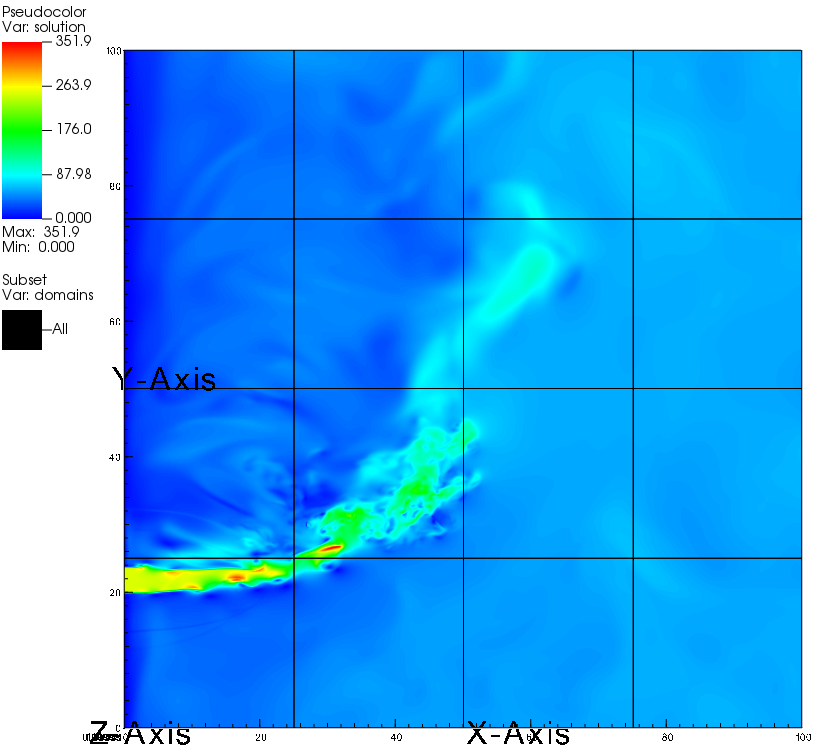
\includegraphics[width=0.45\textwidth]{figures/s3d-2d-profile.png}
	\caption{2-D slice of S3D dataset}
	\label{fig:s3d-adaptive-2d}
\end{figure}

\Remark{show error convergence plots for S3D on 16 subdomains with adaptivity}

\Remark{add table of actual compression and error as $n_s$ is changed}

\Remark{Discuss about complications and potential ways to enforce continuity. (a) Use decoded data, (b) Use control point space across interface}


\subsection{Parallel Scalability}\label{sec:parallel-scalability}

The parallel scalability of the implemented ASM iterative solver for ensuring continuity across block boundaries was measured on the 2-D CESM dataset. Our experiments were executed on the Bebop cluster at
Argonne National Laboratory LCRC (Laboratory Computing Resource Center). Bebop has 1024 public nodes, with Intel Broadwell or Intel Knights Landing processors, with 128 GB memory per Broadwell node, and 104 GB per KNL node. It has an Omni-Path Fabric Interconnect. Broadwell processors have 36 cores, while KNL processors have 64 cores. We primarily used the Broadwell processors for the tests presented below.

\Remark{Showcase strong scalability results on Bebop for the 2-d problem with CESM datasets}
\Remark{How does the nearest neighbor communication stay bounded ? measure timings separately ?}





%\paragraph{Positioning Figures and Tables} Place figures and tables at the top and 
%``Fig.~\ref{fig}'', even at the beginning of a sentence.

%\begin{table}[htbp]
%\caption{Table Type Styles}
%\begin{center}
%\begin{tabular}{|c|c|c|c|}
%\hline
%\textbf{Table}&\multicolumn{3}{|c|}{\textbf{Table Column Head}} \\
%\cline{2-4} 
%\textbf{Head} & \textbf{\textit{Table column subhead}}& \textbf{\textit{Subhead}}& \textbf{\textit{Subhead}} \\
%\hline
%copy& More table copy$^{\mathrm{a}}$& &  \\
%\hline
%\multicolumn{4}{l}{$^{\mathrm{a}}$Sample of a Table footnote.}
%\end{tabular}
%\label{tab1}
%\end{center}
%\end{table}

%\begin{figure}[htbp]
%\centerline{\includegraphics{fig1.png}}
%\caption{Example of a figure caption.}
%\label{fig}
%\end{figure}
